\documentclass[UTF8]{ctexart}
\usepackage[a4paper,margin=2.5cm]{geometry}
\usepackage{amsmath,amssymb}
\usepackage{graphicx}
\usepackage{booktabs}
\usepackage{hyperref}

\title{第七题：基于强化学习的迷宫最短路径搜索}
\author{}
\date{\today}

\begin{document}
\emergencystretch=2em
\maketitle

\section{题目要求}

题目要求利用 Reinforcement Learning 算法求解迷宫最短路径搜索问题。给定迷宫图像
\texttt{maze.jpg}，黄色位置为出发点；用户可以任意给出终点位置，程序需要规划出
最短路径，或者判断该终点不能到达。为满足交互式要求，本解答提供
\texttt{maze\_rl\_gui.py}，可通过鼠标点击或输入栅格坐标设置终点。

\section{图像解析}

迷宫图片中的墙体是带纹理的灰白块，通道是黑色块。程序先从灰白墙体像素自动确定
迷宫边界，再利用边界宽高的最大公约数推断基本块大小。对本图得到：

\begin{center}
\begin{tabular}{ll}
\toprule
项目 & 数值 \\
\midrule
迷宫边界 & $(50,48)$ 到 $(569,439)$ \\
基本块大小 & $8\times 8$ 像素 \\
栅格规模 & $49$ 行 $\times$ $65$ 列 \\
可通行状态数 & $1539$ \\
黄色起点栅格 & $(44,63)$ \\
\bottomrule
\end{tabular}
\end{center}

每个 $8\times 8$ 块被看作一个状态。若该块中灰白墙体像素比例不超过阈值
$0.2$，或该块包含黄色起点像素，则记为可通行状态；否则记为墙体状态。

\begin{figure}[h]
\centering
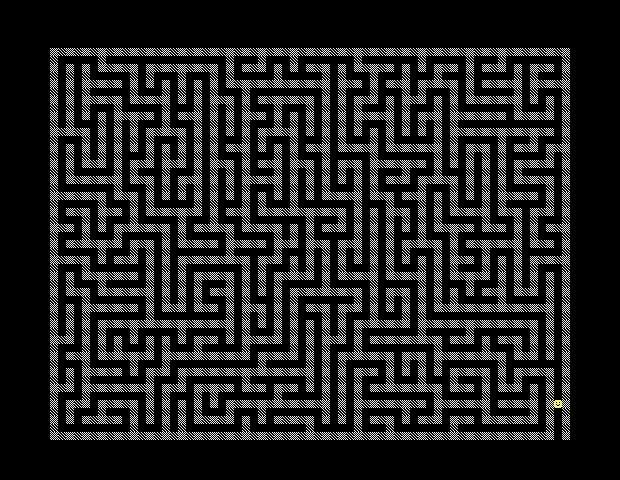
\includegraphics[width=0.75\linewidth]{maze.jpg}
\caption{原始迷宫图像}
\end{figure}

\section{强化学习建模}

将解析后的迷宫表示为确定性 GridWorld：
\begin{itemize}
  \item 状态 $s=(r,c)$ 为一个可通行栅格；
  \item 动作为 $A=\{\mathrm{U},\mathrm{D},\mathrm{L},\mathrm{R}\}$；
  \item 若相邻栅格可通行，则转移到该栅格，否则该动作不作为合法动作；
  \item 终点 $g$ 为吸收状态；
  \item 每走一步奖励为 $-1$，终点价值为 $0$。
\end{itemize}

因此，最优价值函数满足 Bellman 最优方程：
\[
V^*(g)=0,\qquad
V^*(s)=\max_{a\in A(s)}\left[-1+V^*\bigl(T(s,a)\bigr)\right],
\quad s\neq g.
\]

对应的最优动作价值函数为
\[
Q^*(s,a)=-1+V^*\bigl(T(s,a)\bigr),
\qquad
\pi^*(s)=\arg\max_{a\in A(s)}Q^*(s,a).
\]

由于每一步奖励相同且为负数，最大化累计奖励等价于最小化步数。于是
$V^*(s)=-d(s,g)$，其中 $d(s,g)$ 是状态 $s$ 到终点 $g$ 的最短步数。程序采用
从终点反向传播的 Bellman 更新来得到收敛后的 $V^*$ 和 $Q^*$，再从黄色起点按
$Q^*$ 贪心选取动作，从而得到最短路径。

\section{程序使用}

在 \texttt{第7题} 文件夹中运行交互式界面：
\[
\texttt{python maze\_rl\_gui.py}
\]

界面支持两种给定终点的方式：直接在图像上点击目标位置，或输入终点的行列坐标后点击
``求解''。若终点是墙体或在迷宫外，程序会提示不可通行；若可通行，则显示路径和
最短步数。

也可以使用命令行模式复现实验，例如：
\[
\texttt{python maze\_rl\_gui.py --no-gui --goal 1 1 --save goal\_1\_1.png}
\]

\section{运行结果}

命令行测试结果如下：

\begin{center}
\begin{tabular}{lll}
\toprule
终点 & 结果 & 最短步数 \\
\midrule
$(25,33)$ & 可到达，自动示例终点 & $619$ \\
$(1,1)$ & 可到达 & $343$ \\
$(10,10)$ & 位于墙体或不可通行区域 & -- \\
\bottomrule
\end{tabular}
\end{center}

自动示例会选择从起点出发距离最远的可通行终点，并保存路径图
\texttt{demo\_path.png}。实验中，起点为 $(44,63)$，自动终点为 $(25,33)$，
最短路径长度为 $619$ 步，路径共包含 $620$ 个栅格状态。

\begin{figure}[h]
\centering
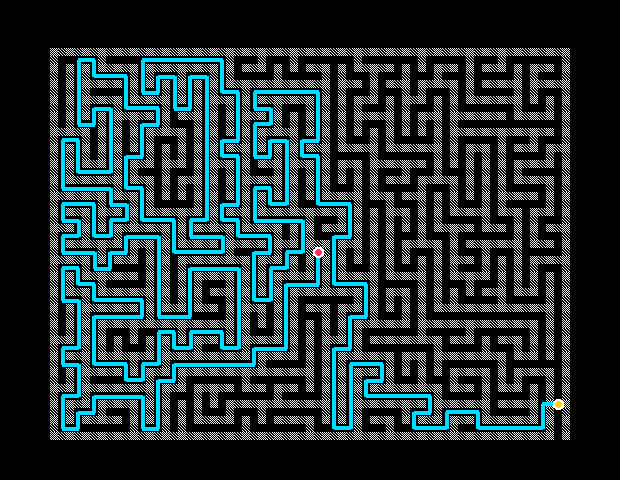
\includegraphics[width=0.75\linewidth]{demo_path.png}
\caption{自动示例终点 $(25,33)$ 的最短路径}
\end{figure}

\section{结论}

该方法将图像迷宫转化为有限状态 MDP，并通过 Bellman 最优方程计算最优
$Q$ 值。由于奖励设计为每步 $-1$，所得最优策略天然对应最短路径；若用户给出的终点
不是可通行状态，程序会直接判断为不能到达。交互式界面可以直观展示不同终点对应的
路径规划结果。

\end{document}
